\documentclass[12pt,a4paper]{book}
\usepackage[utf8]{inputenc}
\usepackage{amsmath,amssymb,amsfonts}
\usepackage{graphicx}
\usepackage[margin=1in]{geometry}
\usepackage{hyperref}
\usepackage{tikz}
\usetikzlibrary{arrows,decorations.markings,patterns,shapes,calc}
\usepackage{pgfplots}
\pgfplotsset{compat=1.17}
\usepackage{enumitem}
\usepackage{float}
\usepackage{makeidx}
\usepackage{mathtools}
\usepackage{bm}
\usepackage{cancel}
\usepackage{fancyhdr}
\usepackage{listings}
\usepackage{color}
\usepackage{multirow}
\usepackage{booktabs}
\pagestyle{fancy}
\fancyhf{}
\fancyhead[L]{\leftmark}
\fancyhead[R]{\thepage}
\renewcommand{\headrulewidth}{0.4pt}

\title{\textbf{Mathematical Modeling and Simulation}\\[5pt]
\Large MATH 521 -- Comprehensive Lecture Notes}
\author{Compiled from S. Banerjee, B. Barnes \& G. R. Fulford, \\ J. N. Kapur, and Giordano et al.}
\date{\today}

\begin{document}
\maketitle
\tableofcontents

\chapter{Introduction to Mathematical Modeling}

\section{What is Mathematical Modeling?}
A mathematical model is a representation, in mathematical terms, of certain aspects of a non‑mathematical system. The process of constructing and analyzing such models is called mathematical modeling. Models serve as bridges between real‑world phenomena and mathematical reasoning; they allow us to understand, predict, and control complex behaviors.

\subsection*{A brief historical perspective}
The roots of mathematical modeling go back to antiquity: Archimedes’ laws of levers, Ptolemy’s planetary motions, and Galileo’s kinematics are early examples. In the 20th century, modeling expanded dramatically with the rise of computing, enabling simulation of nonlinear systems, optimization, and stochastic processes.

\subsection*{Classification of Models}
Models are classified along several dimensions:
\begin{itemize}
    \item \textbf{Deterministic vs. Stochastic}: Deterministic models have no randomness; given the same inputs they always produce the same outputs. Stochastic models incorporate probability, reflecting uncertainty.
    \item \textbf{Static vs. Dynamic}: Static models describe a system at a single instant (e.g., a system of algebraic equations). Dynamic models describe the evolution over time.
    \item \textbf{Discrete vs. Continuous}: Discrete models treat time, state, or space in discrete steps (difference equations, cellular automata). Continuous models use continuous variables and derivatives (differential equations).
    \item \textbf{Lumped vs. Distributed}: Lumped models neglect spatial variation (ordinary differential equations); distributed models explicitly include spatial dependence (partial differential equations).
    \item \textbf{Linear vs. Nonlinear}: Linear models obey the superposition principle; nonlinear ones do not. Nonlinearity often leads to rich phenomena such as multiple equilibria, oscillations, and chaos.
    \item \textbf{Empirical vs. Mechanistic}: Empirical models are based purely on data (curve fitting); mechanistic models are derived from underlying principles (physical laws, biological mechanisms).
\end{itemize}

\section{The Modeling Process}
The modeling process is iterative and can be summarized in the following steps:
\begin{enumerate}[leftmargin=*]
    \item \textbf{Problem identification and formulation:} Understand the real‑world question, define the goals, and specify the system’s boundaries.
    \item \textbf{Make assumptions:} Simplify reality to a tractable set of assumptions; identify variables, parameters, and their relationships. Assumptions must be stated clearly, as they limit the model’s applicability.
    \item \textbf{Mathematical formulation:} Translate assumptions into equations (algebraic, difference, differential, etc.) using physical laws or empirical principles.
    \item \textbf{Solution / analysis:} Solve the equations analytically if possible, or resort to numerical and qualitative methods.
    \item \textbf{Validation:} Compare model predictions with experimental or observational data. If unsatisfactory, re‑examine assumptions and refine the model.
    \item \textbf{Interpretation and prediction:} Use the validated model to answer the original question, make forecasts, or propose experiments.
    \item \textbf{Communication:} Present the model, its limitations, and results to stakeholders.
\end{enumerate}
This cycle (real world $\rightarrow$ mathematical world $\rightarrow$ real world) is often called the \textbf{modeling loop}.

\section{Importance of Mathematical Modeling}
\begin{itemize}[leftmargin=*]
    \item \textbf{Understanding:} Models reveal causal relationships and mechanisms hidden in raw data.
    \item \textbf{Prediction:} They forecast future states (weather, epidemics, stock prices).
    \item \textbf{Optimization \& Control:} Models help design efficient engineering systems, manage resources, and plan strategies.
    \item \textbf{Simulation as experimentation:} Computer simulation of models is often cheaper, faster, and safer than physical experiments.
    \item \textbf{Interdisciplinarity:} The same mathematical structures reappear across disciplines (e.g., logistic growth in ecology, chemistry, and economics).
    \item \textbf{Communication:} A mathematical model provides a precise and unambiguous language for scientific discourse.
\end{itemize}

\section{Limitations of Mathematical Models}
\begin{itemize}[leftmargin=*]
    \item \textbf{Assumptions may be unrealistic:} Simplifications can omit crucial factors, leading to erroneous conclusions.
    \item \textbf{Parameter uncertainty:} Many models rely on parameters that are hard to measure accurately; sensitivity analysis is essential.
    \item \textbf{Trade‑off between complexity and tractability:} Adding realism often makes the model analytically unsolvable and computationally expensive.
    \item \textbf{Validation difficulty:} For many systems (e.g., long‑term climate, economies) controlled experiments are impossible.
    \item \textbf{Chaotic behavior:} In chaotic systems, tiny errors in initial data lead to vastly different predictions (the ``butterfly effect'').
    \item \textbf{Human factors:} Psychological and social behaviors are notoriously difficult to quantify.
    \item \textbf{Misinterpretation:} Users may treat model outputs as exact truths rather than approximations.
\end{itemize}
As the statistician George Box famously said: \textit{“All models are wrong, but some are useful.”}

\section{Illustrative Numerical Examples}
\begin{enumerate}[leftmargin=*, label=\textbf{Example 1.\arabic*}]
    \item \textbf{Bacterial growth – exponential model.}
    A bacterial culture initially contains $N_0 = 500$ cells. After $2$ hours the population is $2000$. Assuming exponential growth $N(t) = N_0 e^{rt}$, estimate the growth rate $r$ and predict the population after $5$ hours.

    \textbf{Solution:}
    From $2000 = 500 e^{2r}$ we obtain $e^{2r} = 4 \;\Rightarrow\; 2r = \ln 4 \;\Rightarrow\; r = \frac{\ln 4}{2} \approx 0.6931\;\text{hr}^{-1}$.
    Then $N(5) = 500 e^{5 \times 0.6931} = 500 e^{3.4655} \approx 500 \times 32 = 16\,000$.

    \item \textbf{Model classification.}
    Classify each of the following models as deterministic or stochastic, static or dynamic, discrete or continuous:
    \begin{enumerate}
        \item $x_{n+1} = k x_n (1 - x_n)$.
        \item $m \frac{d^2x}{dt^2} + c \frac{dx}{dt} + k x = 0$.
        \item A random walk on a line with probability $p$ to step right.
    \end{enumerate}
    \textbf{Solution:}
    \begin{enumerate}
        \item Deterministic, dynamic, discrete (difference equation).
        \item Deterministic, dynamic, continuous (ODE).
        \item Stochastic, dynamic, discrete (if time steps are considered) or continuous‑time depending on framework.
    \end{enumerate}
\end{enumerate}

\section{Exercises}
\begin{enumerate}[leftmargin=*, label=\textbf{Exercise 1.\arabic*}]
    \item Describe the modeling cycle in your own words and illustrate it with the example of modeling the spread of a rumor in a population.
    \item Distinguish between linear and nonlinear models. Give one example of each from population dynamics.
    \item A city had a population of 1.2 million in the year 2010 and 1.5 million in 2020. Assuming an exponential model $P(t)=P_0 e^{rt}$, estimate the annual growth rate and predict the population in 2030. Discuss limitations of this model.
    \item Give two examples of real‑world systems where a discrete model is more appropriate than a continuous model and explain why.
\end{enumerate}

\chapter{Modeling Discrete Processes}
\section{Difference Equations – Basic Concepts}
Many systems are naturally described at discrete time intervals: the annual census of a population, the daily closing price of a stock, the transmission of information in a computer network. Such systems lead to \textbf{difference equations}.

A first‑order difference equation has the form
\[
x_{n+1} = f(n, x_n), \qquad n = 0,1,2,\dots
\]
If $f$ does not depend explicitly on $n$, the equation is \textbf{autonomous}:
\[
x_{n+1} = f(x_n).
\]
An equilibrium (or fixed point) satisfies $x^* = f(x^*)$.

Higher‑order difference equations involve more time indices. An $m$‑th order equation is
\[
x_{n+m} = F(n, x_n, x_{n+1}, \dots, x_{n+m-1}),
\]
and requires $m$ initial conditions $x_0, x_1, \dots, x_{m-1}$ to specify a unique solution.

\subsection*{Examples}
\begin{itemize}
    \item \textbf{Geometric growth:} $x_{n+1} = \lambda x_n$ gives $x_n = \lambda^n x_0$.
    \item \textbf{Arithmetic growth:} $x_{n+1} = x_n + b$ gives $x_n = x_0 + n b$.
    \item \textbf{Fibonacci sequence:} $F_{n+2} = F_{n+1} + F_n$, $F_0=0$, $F_1=1$.
\end{itemize}

\section{Linear Difference Equations}

\subsection{First‑Order Linear Equations}
\[
x_{n+1} = a x_n + b, \quad a,b \;\text{constants}.
\]
\textbf{Solution.} If $b=0$, $x_n = a^n x_0$. If $b\neq0$, a particular constant solution $x^*$ (an equilibrium) must satisfy $x^* = a x^* + b \;\Rightarrow\; x^* = \frac{b}{1-a}$ (provided $a\neq1$). The general solution is the sum of the homogeneous part and the particular solution:
\[
x_n = A a^n + \frac{b}{1-a}.
\]
Using $x_0$ determines $A = x_0 - \frac{b}{1-a}$. Hence
\[
\boxed{x_n = \left(x_0 - \frac{b}{1-a}\right) a^n + \frac{b}{1-a}, \quad a\neq1.}
\]
When $a=1$, $x_{n+1} = x_n + b \;\Rightarrow\; x_n = x_0 + n b$.

\textbf{Stability.} The equilibrium is $x^* = \frac{b}{1-a}$. The sequence converges to $x^*$ as $n\to\infty$ if and only if $|a|<1$. If $|a|>1$, $x_n$ diverges. If $a<0$, the convergence/divergence oscillates in sign.

\subsection{Second‑Order Linear Homogeneous Equations}
\[
x_{n+2} + p x_{n+1} + q x_n = 0.
\]
We seek solutions of the form $x_n = \lambda^n$, which leads to the characteristic equation
\[
\lambda^2 + p\lambda + q = 0.
\]
Depending on the nature of the roots:
\begin{itemize}
    \item \textbf{Real distinct roots} $\lambda_1, \lambda_2$: $x_n = A\lambda_1^n + B\lambda_2^n$.
    \item \textbf{Repeated root} $\lambda$: $x_n = (A + B n) \lambda^n$.
    \item \textbf{Complex conjugate roots} $\lambda = r e^{\pm i\theta}$: $x_n = r^n (A\cos n\theta + B\sin n\theta)$.
\end{itemize}
The constants $A,B$ are found from initial conditions.

\textbf{Example – Fibonacci numbers.}
$F_{n+2} = F_{n+1} + F_n$, so $p=-1$, $q=-1$. Characteristic equation $\lambda^2 - \lambda -1 =0$ gives $\lambda = \frac{1\pm\sqrt{5}}{2}$. The general solution is
\[
F_n = A\left(\frac{1+\sqrt{5}}{2}\right)^n + B\left(\frac{1-\sqrt{5}}{2}\right)^n.
\]
With $F_0=0,F_1=1$, we get $A = 1/\sqrt{5}$, $B = -1/\sqrt{5}$, the famous Binet formula. Since $|\frac{1-\sqrt{5}}{2}| < 1$, the second term decays, and for large $n$, $F_n \approx \frac{1}{\sqrt{5}}\left(\frac{1+\sqrt{5}}{2}\right)^n$, growing like the golden ratio $\phi \approx 1.618$.

\subsection{Systems of Linear Difference Equations}
A $k$‑dimensional linear system is
\[
\mathbf{x}_{n+1} = \mathbf{A} \mathbf{x}_n, \qquad \mathbf{x}_n \in \mathbb{R}^k.
\]
The solution is $\mathbf{x}_n = \mathbf{A}^n \mathbf{x}_0$. Equilibria are $\mathbf{x}^* = \mathbf{0}$ (if $\mathbf{A}-\mathbf{I}$ invertible). Long‑term behaviour depends on the eigenvalues of $\mathbf{A}$:
\begin{itemize}
    \item The zero solution is asymptotically stable if $|\lambda_i| < 1$ for all eigenvalues $\lambda_i$ of $\mathbf{A}$.
    \item It is unstable if any eigenvalue has $|\lambda_i| > 1$.
    \item For complex eigenvalues, the condition is $|\lambda_i| = \sqrt{(\text{Re}\,\lambda_i)^2+(\text{Im}\,\lambda_i)^2} < 1$.
\end{itemize}
If some eigenvalues have modulus exactly $1$, the linear analysis is inconclusive (marginal case).

\textbf{Example – Leslie matrix model.}
A population is divided into age classes. Let $\mathbf{x}_n = (x_{n,1}, x_{n,2}, \dots, x_{n,m})^T$ be the numbers in each class at time $n$. The Leslie matrix is
\[
\mathbf{L} = \begin{pmatrix}
f_1 & f_2 & \dots & f_m \\
s_1 & 0 & \dots & 0 \\
0 & s_2 & \dots & 0 \\
\vdots & \vdots & \ddots & \vdots \\
0 & 0 & \dots & s_{m-1} \! \end{pmatrix},
\]
where $f_i$ are fertilities and $s_i$ are survival rates. Then $\mathbf{x}_{n+1} = \mathbf{L} \mathbf{x}_n$. The dominant eigenvalue $\lambda_1$ (the largest in modulus) determines the asymptotic growth rate; its associated eigenvector gives the stable age distribution.

\section{Nonlinear Difference Equations}

\subsection{Equilibria and Linear Stability}
For $x_{n+1} = f(x_n)$, an equilibrium $x^*$ satisfies $x^* = f(x^*)$. To investigate local stability, let $u_n = x_n - x^*$ be a small perturbation. Taylor expand:
\[
x_{n+1} = f(x^*+u_n) \approx f(x^*) + f'(x^*) u_n = x^* + f'(x^*) u_n,
\]
so $u_{n+1} \approx f'(x^*) u_n$. The multiplier $\lambda = f'(x^*)$ governs the linearized dynamics.
\begin{itemize}
    \item If $|f'(x^*)| < 1$: locally asymptotically stable.
    \item If $|f'(x^*)| > 1$: unstable.
    \item If $|f'(x^*)| = 1$: marginal; higher‑order terms decide.
\end{itemize}
If $f'(x^*) > 0$, convergence/divergence is monotonic; if $f'(x^*) < 0$, it alternates sign.

\subsection{Cobweb Diagrams}
The cobweb diagram is a graphical method to iterate $x_{n+1}=f(x_n)$. On a plane, draw the curve $y = f(x)$ and the line $y=x$. Starting at $(x_0,0)$, go vertically to the curve $(x_0, x_1)$, then horizontally to the diagonal $(x_1,x_1)$, then vertically to $(x_1, x_2)$, and so on. This visualizes convergence to a fixed point, periodic cycles, or chaotic wandering.

\begin{figure}[H]
\centering
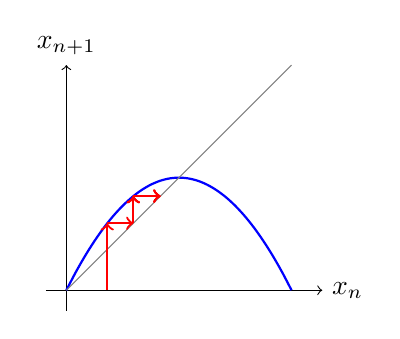
\begin{tikzpicture}[scale=1.3]
\draw[->] (-0.2,0) -- (2.5,0) node[right] {$x_n$};
\draw[->] (0,-0.2) -- (0,2.2) node[above] {$x_{n+1}$};
\draw[domain=0:2.2, smooth, variable=\x, blue, thick] plot ({\x},{2.0*\x*(1-\x/2.2)});
\draw[domain=0:2.2, smooth, gray] plot ({\x},{\x});
\def\xstart{0.4}
\pgfmathsetmacro{\y}{2*\xstart*(1-\xstart/2.2)}
\draw[red, thick, ->] (\xstart,0) -- (\xstart,\y);
\draw[red, thick, ->] (\xstart,\y) -- (\y,\y);
\pgfmathsetmacro{\xnext}{\y}
\foreach \i in {1,...,4}{
\pgfmathsetmacro{\ynext}{2*\xnext*(1-\xnext/2.2)}
\draw[red, thick, ->] (\xnext,\xnext) -- (\xnext,\ynext);
\draw[red, thick, ->] (\xnext,\ynext) -- (\ynext,\ynext);
\pgfmathsetmacro{\xnext}{\ynext}
}
\end{tikzpicture}
\caption{Cobweb for a unimodal map converging to a fixed point.}
\end{figure}

\subsection{The Logistic Map}
The discrete logistic equation (May, 1976) is
\[
x_{n+1} = r x_n (1 - x_n), \qquad x_n \in [0,1],\; 0 \le r \le 4.
\]
This simple nonlinear map exhibits a remarkable range of dynamics.

\subsubsection{Fixed points and their stability}
\begin{align*}
x^* &= 0, \\
x^* &= 1 - \frac{1}{r} \quad (\text{for } r>1).
\end{align*}
Derivative $f'(x) = r(1-2x)$. Thus
\begin{itemize}
    \item At $x^*=0$: $f'(0)=r$. Stable for $0<r<1$, unstable for $r>1$.
    \item At $x^*=1-\frac{1}{r}$: $f'(x^*) = r\bigl(1-2(1-\frac{1}{r})\bigr) = r(1-2+\frac{2}{r}) = 2-r$. This is stable when $|2-r|<1$, i.e. $1<r<3$.
\end{itemize}
At $r=3$, $f'(x^*)=-1$ and the fixed point loses stability via a period‑doubling (flip) bifurcation: a stable 2‑cycle appears.

\subsubsection{Period‑doubling cascade and chaos}
As $r$ increases beyond $3$, the 2‑cycle becomes unstable and a 4‑cycle emerges, then 8, 16, … . The intervals of $r$ for successive period doublings become smaller and converge at $r_\infty \approx 3.5699456$, after which chaotic behavior appears. The ratio of successive interval lengths approaches Feigenbaum’s constant $\delta \approx 4.6692$, a universal feature of the period‑doubling route to chaos.

\subsection{Other Discrete Models}
\begin{itemize}
    \item \textbf{Ricker model} (fisheries): $x_{n+1} = x_n \exp\bigl[r(1 - x_n/K)\bigr]$. Similar period‑doubling behavior.
    \item \textbf{Newton’s method:} $x_{n+1} = x_n - \frac{f(x_n)}{f'(x_n)}$. Roots are super‑stable fixed points.
    \item \textbf{SIR discrete‑time models} with generation intervals (e.g., measles epidemics).
\end{itemize}

\section{Solved Examples}
\begin{enumerate}[leftmargin=*, label=\textbf{Example 2.\arabic*}]
    \item \textbf{Solving a first‑order linear equation.}
    $x_{n+1} = 0.5 x_n + 3$, $x_0 = 2$. Find $x_n$, equilibrium, stability.

    \textbf{Solution:} $a=0.5, b=3$, equilibrium $x^* = 3/(1-0.5)=6$.
    $x_n = (2-6)(0.5)^n + 6 = -4(0.5)^n + 6$.
    As $n\to\infty$, $x_n \to 6$ because $|0.5|<1$. Stable.

    \item \textbf{Second‑order linear difference equation.}
    Solve $x_{n+2} - 3 x_{n+1} + 2 x_n = 0$ with $x_0=1, x_1=3$.

    \textbf{Solution:} Characteristic equation $\lambda^2 -3\lambda +2 =0$ $\Rightarrow$ $\lambda=1,2$.
    General solution $x_n = A\cdot 1^n + B\cdot 2^n = A + B\cdot 2^n$.
    Using $x_0=1$: $A+B=1$. $x_1=3$: $A+2B=3$. Solving gives $A=-1$, $B=2$. Thus $x_n = -1 + 2^{n+1}$. (Check: $n=0$: $-1+2=1$; $n=1$: $-1+4=3$.)

    \item \textbf{Leslie matrix growth rate.}
    A population has two age classes: juveniles (class 1) and adults (class 2). Each adult produces on average 2 juveniles per year; 50\% of juveniles survive to become adults; 80\% of adults survive yearly. Find the Leslie matrix and the long‑term growth rate.

    \textbf{Solution:}
    \[
    \mathbf{L} = \begin{pmatrix} 0 & 2 \\ 0.5 & 0.8 \end{pmatrix}.
    \]
    Characteristic polynomial: $\det(\mathbf{L} - \lambda \mathbf{I}) = \lambda^2 - 0.8\lambda - 1 = 0$ $\Rightarrow$ $\lambda = \frac{0.8 \pm \sqrt{0.64+4}}{2} = \frac{0.8 \pm 2.154}{2}$.
    The dominant eigenvalue is $\lambda_1 \approx 1.477$, so population grows about $47.7\%$ per year.

    \item \textbf{Logistic map stability.}
    For $r=2.5$, find the non‑zero fixed point and classify.

    \textbf{Solution:} $x^* = 1 - 1/2.5 = 0.6$. $f'(0.6) = 2.5(1-1.2) = -0.5$. $|f'(0.6)|=0.5<1$ $\Rightarrow$ stable; oscillations in sign because derivative negative.

    \item \textbf{Cobweb of a cubic map.}
    Show that for $x_{n+1} = -x_n^3$, $|x_0|<1$ leads to convergence to $0$, while $|x_0|>1$ diverges.

    \textbf{Solution:} $f(x)=-x^3$. Fixed point $x^*=0$, $f'(0)=0$ (super‑stable). For $|x_0|<1$, $|x_{n+1}| = |x_n|^3$, so magnitude shrinks extremely fast; sequence alternates sign. For $|x_0|>1$, $|x_n| \to \infty$.

    \item \textbf{Ricker model.}
    $x_{n+1} = x_n e^{r(1-x_n)}$, $r=1.5$. Find equilibria and stability.

    \textbf{Solution:} Equilibria: $x^*=0$, and $x^*=1$ (since $e^{r(1-x)}=1$ $\Rightarrow$ $r(1-x)=0$). $f'(x) = e^{r(1-x)}(1 - r x)$.
    At $0$: $f'(0)=e^r >1$ (unstable). At $1$: $f'(1)=e^0(1-1.5) = -0.5$, $|f'|=0.5<1$ (stable).
\end{enumerate}

\section{Exercises}
\begin{enumerate}[leftmargin=*, label=\textbf{Exercise 2.\arabic*}]
    \item Solve $x_{n+1} = -2 x_n + 5$, $x_0=1$. Is the equilibrium stable?
    \item Find all fixed points of $x_{n+1} = x_n^2 - 2$ and determine their stability.
    \item The sequence $x_{n+2} = 4 x_{n+1} - 4 x_n$ with $x_0=2, x_1=3$. Find an explicit formula.
    \item A Leslie matrix is $\mathbf{L} = \begin{pmatrix} 0 & 3 & 2 \\ 0.2 & 0 & 0 \\ 0 & 0.5 & 0 \end{pmatrix}$. Find the dominant eigenvalue and the stable age distribution.
    \item For the logistic map with $r=3.2$, compute the first 20 iterates from $x_0=0.5$. What pattern do you observe?
    \item Investigate the map $x_{n+1} = 1 - a x_n^2$ (the “tent‑like” logistic). Determine the fixed points and find the value of $a$ where a period‑2 cycle appears.
    \item (Research) Discuss how the Fibonacci sequence appears in phyllotaxis and the arrangement of sunflower seeds.
\end{enumerate}

\chapter{Continuous Models Using Ordinary Differential Equations}
\section{Formation of Various Continuous Models}
\subsection{Population Dynamics of a Single Species}
\textbf{Malthusian growth.} If the per capita growth rate is constant $r$, then
\[
\frac{dN}{dt} = r N, \quad N(0)=N_0 \;\Longrightarrow\; N(t) = N_0 e^{rt}.
\]
This is suitable only for short times or unlimited resources.

\textbf{Logistic growth.} The per capita growth rate decreases linearly with population size:
\[
\frac{dN}{dt} = r N \left(1 - \frac{N}{K}\right),
\]
where $K>0$ is the carrying capacity. The closed‑form solution is
\[
N(t) = \frac{K N_0 e^{rt}}{K + N_0 (e^{rt} - 1)}.
\]
The equilibrium $N=K$ is globally stable; $N=0$ is unstable if $r>0$.

\textbf{Harvesting models.}
\begin{itemize}
    \item Constant yield: $\displaystyle \frac{dN}{dt} = r N(1 - N/K) - H$.
    \item Constant effort: $\displaystyle \frac{dN}{dt} = r N(1 - N/K) - q E N$, where $E$ is effort.
\end{itemize}
These can have multiple equilibria and bifurcations.

\textbf{Allee effect.} For some species, growth rate is negative at low densities (e.g., difficulty in finding mates).
\[
\frac{dN}{dt} = r N \left(1 - \frac{N}{K}\right)(N - A), \quad 0 < A < K.
\]
$N=0$ and $N=K$ are stable, $N=A$ is an unstable threshold.

\subsection{Interacting Populations}
\textbf{Lotka–Volterra predator–prey.}
\begin{align*}
\frac{dN}{dt} &= r N - a N P,\\
\frac{dP}{dt} &= b N P - m P.
\end{align*}
Equilibria: $(0,0)$ (saddle) and $\bigl(\frac{m}{b}, \frac{r}{a}\bigr)$ (center). The system has a first integral and neutral cycles; structural instability means small changes (e.g., carrying capacity for prey) can change the center to a stable focus or limit cycle.

\textbf{Competition.}
\begin{align*}
\frac{dN_1}{dt} &= r_1 N_1 \left(1 - \frac{N_1}{K_1} - \alpha_{12} \frac{N_2}{K_1}\right),\\
\frac{dN_2}{dt} &= r_2 N_2 \left(1 - \frac{N_2}{K_2} - \alpha_{21} \frac{N_1}{K_2}\right).
\end{align*}
Four outcomes are possible depending on the relative strength of inter‑ vs. intraspecific competition: coexistence, competitive exclusion of one species, or bistability.

\textbf{Mutualism, symbiosis, and other interactions} can be modeled similarly.

\subsection{Epidemic Models}
The classical Kermack–McKendrick SIR model for a directly transmitted disease:
\begin{align*}
\frac{dS}{dt} &= -\beta S I,\\
\frac{dI}{dt} &= \beta S I - \gamma I,\\
\frac{dR}{dt} &= \gamma I.
\end{align*}
Total population $N = S + I + R$ is constant. The basic reproduction number is $\mathcal{R}_0 = \frac{\beta N}{\gamma}$. If $\mathcal{R}_0 > 1$, an epidemic occurs; the peak fraction of infected can be computed. No long‑term oscillations; the epidemic eventually dies out leaving a fraction of susceptibles.

\subsection{Mechanical Systems}
\textbf{Spring–mass–damper:}
$m \ddot{x} + c \dot{x} + k x = 0$, which as a first‑order system is
\begin{align*}
\dot{x} &= v,\\
\dot{v} &= -\frac{k}{m} x - \frac{c}{m} v.
\end{align*}
Equilibrium $(0,0)$ can be a node, spiral, or center depending on damping.

\textbf{Simple pendulum:} $\ddot{\theta} + \frac{g}{L} \sin\theta = 0$. Equilibria: $\theta = 0$ (stable center in undamped case), $\theta = \pi$ (saddle).

\subsection{Chemical Kinetics}
The law of mass action leads to ODE systems. For the autocatalytic reaction $A + X \to 2X$, $X \to Y$, one may obtain the Lotka–Volterra system or more complex oscillations (e.g., Brusselator, Oregonator).

\section{Linearization and Stability Analysis}

\subsection{Autonomous Systems and Equilibria}
Consider $\dot{\mathbf{x}} = \mathbf{F}(\mathbf{x})$, $\mathbf{x}\in\mathbb{R}^n$. A point $\mathbf{x}^*$ is an equilibrium if $\mathbf{F}(\mathbf{x}^*) = \mathbf{0}$.

\subsection{Linearization around an Equilibrium}
Set $\mathbf{x} = \mathbf{x}^* + \mathbf{u}$, with $\|\mathbf{u}\|$ small. Expanding in Taylor series:
\[
\dot{\mathbf{u}} = \mathbf{F}(\mathbf{x}^* + \mathbf{u}) \approx \mathbf{F}(\mathbf{x}^*) + \mathbf{J}(\mathbf{x}^*) \mathbf{u} = \mathbf{J}(\mathbf{x}^*) \mathbf{u},
\]
where $\mathbf{J}$ is the Jacobian matrix with entries $J_{ij} = \frac{\partial F_i}{\partial x_j}$. The linearized system $\dot{\mathbf{u}} = \mathbf{J}\mathbf{u}$ determines the local behavior, provided $\mathbf{x}^*$ is \textbf{hyperbolic} (no eigenvalue of $\mathbf{J}$ lies on the imaginary axis). This is the content of the Hartman–Grobman theorem.

\subsection{Classification of Equilibria in 2D}
For a $2\times2$ matrix $\mathbf{A}$ with trace $\tau = \text{tr}(\mathbf{A})$ and determinant $\Delta = \det(\mathbf{A})$, the eigenvalues are the roots of $\lambda^2 - \tau\lambda + \Delta = 0$. The nature of the equilibrium is:
\begin{itemize}
    \item $\Delta < 0$: saddle point (real eigenvalues of opposite sign).
    \item $\Delta > 0$:
    \begin{itemize}
        \item $\tau^2 - 4\Delta > 0$: node (real, same sign). Stable if $\tau<0$, unstable if $\tau>0$.
        \item $\tau^2 - 4\Delta < 0$: spiral (complex conjugate). Stable if $\tau<0$, unstable if $\tau>0$.
        \item $\tau = 0$, $\tau^2 - 4\Delta < 0$: center (linearized) — nonlinear terms decide actual behavior.
    \end{itemize}
    \item $\Delta = 0$: at least one zero eigenvalue — degenerate case.
\end{itemize}
The eigenvectors determine the stable/unstable manifolds for saddles.

\subsection{Lyapunov's Indirect Method}
If the Jacobian has all eigenvalues with negative real parts, the equilibrium is asymptotically stable. If any eigenvalue has positive real part, it is unstable.

\section{Bifurcations in ODEs}
A bifurcation is a qualitative change in the phase portrait as a parameter is varied. Normal forms capture the essential dynamics near the bifurcation point.

\subsection{Saddle‑Node Bifurcation}
Normal form: $\dot{x} = r + x^2$ (or $r - x^2$). For $r<0$, two equilibria $\pm\sqrt{-r}$ (one stable, one unstable). At $r=0$, they coalesce into a semi‑stable point. For $r>0$, no equilibria. This bifurcation occurs when a parameter change causes the annihilation of a pair of equilibria.

\textbf{Example:} $\dot{N} = rN(1 - N/K) - H$. As $H$ increases, the two positive equilibria move together and disappear at a critical harvesting rate $H_c$ (saddle‑node).

\subsection{Transcritical Bifurcation}
Normal form: $\dot{x} = r x - x^2$. Equilibria $x=0$ and $x=r$ exchange stability at $r=0$. Typically occurs when an equilibrium never disappears but changes stability.

\textbf{Example:} In the logistic equation with varying $r$ sign, or in models with a simple Allee effect.

\subsection{Pitchfork Bifurcation}
\textbf{Supercritical:} $\dot{x} = r x - x^3$. For $r<0$, only stable $x=0$. For $r>0$, $x=0$ becomes unstable and two stable equilibria $\pm\sqrt{r}$ appear. This models symmetry‑breaking.

\textbf{Subcritical:} $\dot{x} = r x + x^3$. The bifurcating branches for $r<0$ are unstable, leading to sudden jumps.

\textbf{Example:} Buckling of a beam, or population with strong Allee effect where the threshold can appear/disappear.

\subsection{Hopf Bifurcation}
In 2D (or higher), a pair of complex conjugate eigenvalues crosses the imaginary axis with non‑zero speed. A limit cycle is born (or destroyed). Normal form in polar coordinates:
\begin{align*}
\dot{r} &= \mu r - r^3 \quad \text{(supercritical)},\\
\dot{\theta} &= \omega.
\end{align*}
For $\mu<0$, stable focus at origin. At $\mu=0$, Hopf bifurcation. For $\mu>0$, unstable focus and a stable limit cycle of radius $\sqrt{\mu}$.

\textbf{Example:} Predator–prey with prey carrying capacity; as $K$ increases, the equilibrium loses stability via Hopf, leading to sustained oscillations.

\section{Solved Examples}
\begin{enumerate}[leftmargin=*, label=\textbf{Example 3.\arabic*}]
    \item \textbf{Logistic solution.}
    Solve $\frac{dN}{dt} = 0.2 N(1 - N/1000)$ with $N(0)=100$. Find $N(10)$.

    \textbf{Solution:} $r=0.2, K=1000$. Formula:
    $N(t) = \frac{1000 \cdot 100 e^{0.2t}}{1000 + 100(e^{0.2t}-1)} = \frac{100000 e^{0.2t}}{900 + 100 e^{0.2t}}$.
    At $t=10$, $e^2 \approx 7.389$, $N(10) = \frac{1000 \times 7.389}{9 + 7.389} = \frac{7389}{16.389} \approx 450.8$.

    \item \textbf{Lotka–Volterra equilibria.}
    For $\dot{N}=0.5N - 0.01 N P$, $\dot{P}=0.001 N P - 0.2 P$, find equilibria and classify.

    \textbf{Solution:}
    \begin{align*}
        (0,0):\; \mathbf{J} = \begin{pmatrix}0.5 & 0 \\ 0 & -0.2\end{pmatrix}, \; \lambda=0.5,-0.2 \;\text{(saddle)}.
    \end{align*}
    Coexistence: $N^* = \frac{0.2}{0.001}=200$, $P^* = \frac{0.5}{0.01}=50$. Jacobian:
    \[
    \mathbf{J} = \begin{pmatrix} 0.5-0.01 P & -0.01 N \\ 0.001 P & 0.001 N - 0.2 \end{pmatrix} = \begin{pmatrix} 0 & -2 \\ 0.05 & 0 \end{pmatrix}.
    \]
    $\tau=0$, $\Delta=0.1>0$ $\Rightarrow$ center in linearization. Nonlinear system has a family of periodic orbits (conservative).

    \item \textbf{SIR model peak.}
    With $\beta=0.001, \gamma=0.1$, $N=1000$, $S_0=999, I_0=1$. Compute $\mathcal{R}_0$, show epidemic, find $I_{\max}$.

    \textbf{Solution:} $\mathcal{R}_0 = \frac{\beta N}{\gamma} = \frac{1}{0.1}=10>1$. Epidemic. The curve in the $(S,I)$ plane: $\frac{dI}{dS} = -1 + \frac{\gamma}{\beta S}$ $\Rightarrow$ $I = -S + \frac{\gamma}{\beta}\ln S + C$.
    Using $(999,1)$: $C = 1 + 999 - 100 \ln 999 \approx 1000 - 100\times 6.9078 = 309.22$.
    Peak when $S = \gamma/\beta = 100$, then $I_{\max} = -100 + 100\ln 100 + 309.22 \approx -100 + 460.52 + 309.22 = 669.74$.

    \item \textbf{Saddle‑node in harvesting.}
    $\dot{N} = 0.5 N(1 - N/100) - H$. Find $H_c$ where positive equilibria disappear.

    \textbf{Solution:} Equilibria satisfy $0.005 N^2 - 0.5 N + H = 0$. $N = 50 \pm \sqrt{2500 - 200 H}$.
    For real roots, $2500 - 200H \ge 0 \Rightarrow H \le 12.5$. At $H_c=12.5$, semi‑stable at $N=50$.

    \item \textbf{Supercritical pitchfork.}
    $\dot{x} = \mu x - x^3$. For $\mu<0$, only $x=0$ stable; for $\mu>0$, $x=0$ unstable, $x=\pm\sqrt{\mu}$ stable.

    \item \textbf{Hopf bifurcation example.}
    In polar form: $\dot{r} = \mu r - r^3$, $\dot{\theta} = \omega$. Show supercritical Hopf at $\mu=0$.

    \textbf{Solution:} For $\mu<0$, the only critical point is $r=0$ (stable focus). At $\mu=0$, the origin is weakly attracting; for $\mu>0$, $r=0$ unstable and a stable limit cycle of radius $\sqrt{\mu}$ appears. Hence a supercritical Hopf bifurcation.
\end{enumerate}

\section{Exercises}
\begin{enumerate}[leftmargin=*, label=\textbf{Exercise 3.\arabic*}]
    \item Solve $\frac{dN}{dt} = 0.8 N \left(1 - \frac{N}{500}\right)$ with $N(0)=50$. When does $N$ reach $250$?
    \item For the competition model
    \begin{align*}
    \dot{x} &= x(2 - x - y),\\
    \dot{y} &= y(1 - 0.5 x - y),
    \end{align*}
    find all equilibria, classify them, and sketch the phase portrait.
    \item Damped pendulum: $\ddot{\theta} + b \dot{\theta} + \frac{g}{L} \sin\theta = 0$. Write as system, find equilibria, linearize about $(0,0)$, discuss stability as a function of $b$.
    \item Consider the SIR model with vital dynamics (births and deaths): $\dot{S} = \mu N - \beta S I - \mu S$, $\dot{I} = \beta S I - (\gamma + \mu) I$, $\dot{R} = \gamma I - \mu R$. Find the disease‑free equilibrium and the basic reproduction number $\mathcal{R}_0$.
    \item Determine the type of bifurcation at $r=0$ for $\dot{x} = r x + x^2 - x^3$.
    \item (Computational) Simulate the Lorenz system $\dot{x} = 10(y-x)$, $\dot{y} = x(28-z)-y$, $\dot{z} = xy - \tfrac{8}{3}z$ using a simple Euler method with step $0.01$. Plot the trajectory and note the chaotic attractor.
\end{enumerate}

\chapter{Spatial Models Using Partial Differential Equations}
\section{Derivation of the Diffusion Equation}
Consider a substance distributed along a line, with concentration $u(x,t)$. The flux $\mathbf{J}(x,t)$ is the amount crossing a point per unit time. \textbf{Fick’s law} states that the flux is proportional to the negative gradient of concentration:
\[
\mathbf{J} = -D \frac{\partial u}{\partial x},
\]
where $D>0$ is the diffusion coefficient. Conservation of mass for an arbitrary segment $[a,b]$ gives
\[
\frac{d}{dt} \int_a^b u(x,t)\,dx = \mathbf{J}(a,t) - \mathbf{J}(b,t) = -\int_a^b \frac{\partial \mathbf{J}}{\partial x}\,dx.
\]
Thus $\frac{\partial u}{\partial t} + \frac{\partial \mathbf{J}}{\partial x} = 0$. Substituting Fick’s law gives the 1D diffusion (heat) equation:
\[
\frac{\partial u}{\partial t} = D \frac{\partial^2 u}{\partial x^2}.
\]
In higher dimensions, $u_t = D \nabla^2 u$.

\subsection{Random Walk Derivation}
Alternatively, consider particles performing a symmetric random walk on a 1D lattice with spacing $\Delta x$ and time step $\Delta t$. The probability $p(x,t)$ satisfies
\[
p(x,t+\Delta t) = \frac{1}{2} p(x-\Delta x,t) + \frac{1}{2} p(x+\Delta x,t).
\]
Expanding in Taylor series and taking $\Delta x, \Delta t \to 0$ with $D = (\Delta x)^2/(2\Delta t)$ constant yields the diffusion equation.

\section{Reaction–Diffusion Models}
When local kinetics (reactions) are combined with diffusion, we obtain reaction–diffusion equations:
\[
\frac{\partial u}{\partial t} = D \nabla^2 u + f(u).
\]
\textbf{Fisher–KPP equation} (1937):
\[
u_t = D u_{xx} + r u (1 - u).
\]
It supports traveling wave solutions $u(x,t) = U(z)$, $z = x - ct$, connecting the stable equilibrium $U=1$ to the unstable $U=0$. The minimum wave speed is $c_{\min} = 2\sqrt{rD}$.

\section{Linear Stability Analysis for PDEs}

\subsection{Stability of Homogeneous Steady State}
Suppose $u^*$ satisfies $f(u^*) = 0$. Linearizing $u = u^* + \epsilon v(x,t)$ gives
\[
v_t = D v_{xx} + f'(u^*) v.
\]
Assume a Fourier mode $v(x,t) = e^{\lambda t} e^{i k x}$. Substitution yields the dispersion relation
\[
\lambda = f'(u^*) - D k^2.
\]
Thus:
\begin{itemize}
    \item If $f'(u^*) < 0$, then $\lambda < 0$ for all $k$; the steady state is stable against all perturbations.
    \item If $f'(u^*) > 0$, the mode with wavenumber $k$ is unstable if $D k^2 < f'(u^*)$. The most unstable (largest growth rate) occurs at $k=0$, i.e., homogeneous perturbation.
\end{itemize}

\subsection{Turing Instability (Diffusion‑Driven Instability)}
Consider a two‑species system:
\begin{align*}
u_t &= D_u u_{xx} + f(u,v),\\
v_t &= D_v v_{xx} + g(u,v).
\end{align*}
Let $(u^*,v^*)$ be a homogeneous steady state that is stable in the absence of diffusion, i.e., the Jacobian $\mathbf{J} = \begin{pmatrix} f_u & f_v \\ g_u & g_v \end{pmatrix}$ has $\text{tr}(\mathbf{J}) < 0$ and $\det(\mathbf{J}) > 0$. With diffusion, we consider perturbations $e^{\lambda t + i k x}$ and obtain the characteristic equation
\[
\lambda^2 + \lambda\bigl[k^2(D_u+D_v) - \text{tr}(\mathbf{J})\bigr] + h(k^2) = 0,
\]
where
\[
h(k^2) = D_u D_v k^4 - (D_v f_u + D_u g_v) k^2 + \det(\mathbf{J}).
\]
A Turing instability occurs if $h(k^2) < 0$ for some $k \neq 0$, which leads to $\lambda$ real and positive. Necessary conditions:
\begin{enumerate}
    \item $f_u + g_v < 0$ (stable without diffusion),
    \item $f_u g_v - f_v g_u > 0$,
    \item $D_v f_u + D_u g_v > 0$,
    \item $(D_v f_u + D_u g_v)^2 - 4 D_u D_v \det(\mathbf{J}) > 0$.
\end{enumerate}
Typically this requires $D_v \gg D_u$ (a fast‑diffusing inhibitor and a slow‑diffusing activator). The system then forms spatial patterns (Turing patterns) such as spots and stripes.

\section{Research Problems in Spatial Models}
\begin{itemize}
    \item \textbf{Morphogenesis:} Turing’s original paper (1952) proposed reaction–diffusion as a mechanism for biological pattern formation (zebra stripes, leopard spots).
    \item \textbf{Traveling waves in excitable media:} FitzHugh–Nagumo model for nerve impulses; propagating fronts in forest fires, epidemic waves.
    \item \textbf{Chemotaxis:} Keller–Segel model for cell aggregation, with possible blow‑up.
    \item \textbf{Invasion speeds:} How fast does an invasive species spread? Fisher–KPP waves.
    \item \textbf{Vegetation patterns:} Tiger bush in arid ecosystems.
    \item \textbf{Pattern formation in chemical systems:} Belousov–Zhabotinsky reaction.
\end{itemize}

\section{Solved Examples}
\begin{enumerate}[leftmargin=*, label=\textbf{Example 4.\arabic*}]
    \item \textbf{Heat equation on a ring.}
    Solve $u_t = D u_{xx}$ on $[0,L]$ with periodic BC and initial condition $u(x,0) = \cos(2\pi x/L)$.

    \textbf{Solution:} The initial profile is an eigenfunction: $k = 2\pi/L$, solution $u(x,t) = e^{-D k^2 t} \cos(k x)$. It decays exponentially with rate $D k^2$.

    \item \textbf{Fisher wave speed.}
    For $u_t = u_{xx} + u(1-u)$, find $c_{\min}$.

    \textbf{Solution:} $D=1, r=1$ $\Rightarrow$ $c_{\min} = 2\sqrt{1\cdot1} = 2$.

    \item \textbf{Turing conditions in Schnakenberg model.}
    (Dimensionless) $u_t = D_u u_{xx} + \gamma(a - u + u^2 v)$, $v_t = D_v v_{xx} + \gamma(b - u^2 v)$.
    With $a=0.1, b=0.9, \gamma=1$, find homogeneous steady state, Jacobian, and check for Turing instability when $D_u=1, D_v=10$.

    \textbf{Solution:} Homogeneous equilibrium: $a - u + u^2 v = 0$, $b - u^2 v = 0$ $\Rightarrow$ $v = b/u^2$, $a - u + b = 0 \Rightarrow u = a+b = 1.0$, $v = 0.9$.
    Jacobian: $f_u = -1 + 2u v = -1 + 1.8 = 0.8$, $f_v = u^2 = 1$, $g_u = -2u v = -1.8$, $g_v = -u^2 = -1$.
    Trace $= 0.8 - 1 = -0.2 < 0$, determinant $= (0.8)(-1) - (1)(-1.8) = -0.8+1.8 = 1.0 > 0$ $\Rightarrow$ stable without diffusion.
    Now $D_v f_u + D_u g_v = 10(0.8) + 1(-1) = 7 > 0$; $(7)^2 - 4\cdot1\cdot10\cdot1 = 49 - 40 = 9 > 0$. So Turing instability possible for a range of $k$.

    \item \textbf{Linear stability of $u^*=0$ in Fisher.}
    $u_t = D u_{xx} + r u(1-u)$, $u^*=0$, $f'(0)=r$. $\lambda = r - D k^2$. Unstable for $k^2 < r/D$.
\end{enumerate}

\section{Exercises}
\begin{enumerate}[leftmargin=*, label=\textbf{Exercise 4.\arabic*}]
    \item Solve $u_t = 0.1 u_{xx}$ on $[0,\pi]$ with BC $u(0)=u(\pi)=0$ and $u(x,0)=\sin(2x)$. Determine $u(x,t)$.
    \item Derive the Fisher–KPP equation from a population model with logistic growth and random dispersal.
    \item For the Brusselator model:
    \begin{align*}
    u_t &= D_u u_{xx} + A - (B+1)u + u^2 v,\\
    v_t &= D_v v_{xx} + B u - u^2 v,
    \end{align*}
    with $A=1, B=3$. Find homogeneous equilibrium, Jacobian, and conditions for Turing instability.
    \item Using separation of variables, solve the 2D heat equation $u_t = \alpha (u_{xx}+u_{yy})$ on a rectangle $[0,a]\times[0,b]$ with Dirichlet zero BC. Write the solution as a double Fourier series.
    \item (Research) Summarize Turing’s theory of morphogenesis and its limitations.
\end{enumerate}

\chapter{Modeling with Delay Differential Equations}
\section{Introduction to Delay Differential Equations}
Many processes involve a time lag between cause and effect. Maturation periods, incubation times, transport delays lead to \textbf{delay differential equations (DDEs)}. The simplest form with one constant delay $\tau>0$ is
\[
\frac{dx}{dt} = f\bigl(t, x(t), x(t-\tau)\bigr).
\]
The state at time $t$ depends on the state at time $t-\tau$. To obtain a unique solution, we must specify a \textbf{history function} on $[-\tau, 0]$:
\[
x(t) = \phi(t), \quad t \in [-\tau, 0].
\]
The method of steps can be used to construct solutions by solving a sequence of ODEs on intervals of length $\tau$.

\section{Models Using Delay Differential Equations}
\subsection{Hutchinson’s Equation (Delayed Logistic)}
\[
\frac{dN}{dt} = r N(t) \left(1 - \frac{N(t-\tau)}{K}\right).
\]
The regulatory effect depends on population $\tau$ units ago. Equilibrium $N^*=K$; linearized stability reveals that if $\tau$ is small, $N^*$ is stable, but as $\tau$ increases past a critical value, the equilibrium destabilizes via a Hopf bifurcation, leading to oscillations.

\subsection{Nicholson’s Blowflies}
\[
\frac{dN}{dt} = P N(t-\tau) e^{-a N(t-\tau)} - \delta N(t).
\]
This model was fitted to experimental data on blowfly populations and exhibits stable cycles for certain parameters.

\subsection{Mackey–Glass Equation}
\[
\frac{dP}{dt} = \frac{\beta \theta^n P(t-\tau)}{\theta^n + P(t-\tau)^n} - \gamma P(t).
\]
Used to model blood cell production. Depending on parameters, it can show steady states, periodic oscillations, and chaos (for large delays).

\subsection{Epidemic Models with Latency (SEIR)}
Incorporating an exposed (latent) period $\tau$:
\[
\frac{dS}{dt} = -\beta S(t) I(t),\quad
\frac{dE}{dt} = \beta S(t) I(t) - \beta S(t-\tau) I(t-\tau) e^{-\mu \tau},
\]
\[
\frac{dI}{dt} = \beta S(t-\tau) I(t-\tau) e^{-\mu \tau} - (\mu+\gamma) I(t),
\]
where $e^{-\mu\tau}$ accounts for death during the latent period.

\section{Linear Stability Analysis for DDEs}
Consider an equilibrium $x^*$ of $\dot{x} = f(x(t), x(t-\tau))$. Linearize by setting $x(t) = x^* + u(t)$:
\[
\dot{u}(t) = a u(t) + b u(t-\tau),
\]
where $a = \frac{\partial f}{\partial x(t)}$, $b = \frac{\partial f}{\partial x(t-\tau)}$ evaluated at $(x^*,x^*)$. Seeking solutions $u(t) = e^{\lambda t}$ yields the characteristic equation:
\[
\lambda = a + b e^{-\lambda \tau}.
\]
This transcendental equation has infinitely many complex roots. The equilibrium is asymptotically stable if all roots satisfy $\text{Re}(\lambda) < 0$.

\subsection{No Delay ($\tau=0$)}
Then $\lambda = a + b$, stability requires $a+b < 0$.

\subsection{Effect of Delay}
As $\tau$ increases, pairs of complex conjugate roots may cross the imaginary axis, leading to a Hopf bifurcation. To find the critical delay $\tau_c$, set $\lambda = i\omega$ ($\omega > 0$):
\[
i\omega = a + b (\cos \omega\tau - i \sin \omega\tau).
\]
Separate real and imaginary parts:
\[
0 = a + b \cos \omega\tau, \qquad \omega = -b \sin \omega\tau.
\]
Squaring and adding yields
\[
\omega^2 = b^2 - a^2.
\]
Thus a necessary condition for oscillatory instability is $b^2 > a^2$. The critical delay is then
\[
\tau_c = \frac{1}{\omega} \arccos\!\left(-\frac{a}{b}\right) + \frac{2\pi n}{\omega}, \quad n=0,1,2,\dots
\]
The smallest positive $\tau_c$ (usually $n=0$) gives the first Hopf bifurcation.

\subsection{Example: Delayed Logistic Equation (Hutchinson)}
Dimensionless form: $\dot{x} = r x(t) [1 - x(t-\tau)]$. Equilibrium $x^*=1$. Linearize by writing $x=1+u$; then $\dot{u} \approx -r u(t-\tau)$. So $a=0$, $b=-r$. Then $\omega^2 = r^2$, $\omega = r$. $\cos(\omega\tau_c) = -a/b = 0$, so $\omega\tau_c = \frac{\pi}{2}$, giving $\tau_c = \frac{\pi}{2r}$. For $\tau < \tau_c$, equilibrium stable; for $\tau > \tau_c$, stable limit cycle exists.

\section{Solved Examples}
\begin{enumerate}[leftmargin=*, label=\textbf{Example 5.\arabic*}]
    \item \textbf{Method of steps.}
    Solve $\dot{x}(t) = -x(t-1)$ for $t\ge0$ with history $x(t)=2$ on $[-1,0]$.

    \textbf{Solution:}
    On $[0,1]$: $x(t-1)=2$, so $\dot{x} = -2$, $x(t) = 2 - 2t$.
    On $[1,2]$: $x(t-1) = 2 - 2(t-1) = 4 - 2t$, $\dot{x} = -(4-2t) = 2t-4$, $x(t) = t^2 - 4t + C$. Continuity at $t=1$: $x(1)=0 \Rightarrow 1 -4 + C = 0 \Rightarrow C=3$, so $x(t) = t^2 -4t + 3$.

    \item \textbf{Hutchinson’s equation critical delay.}
    For $\dot{N} = 0.5 N(t) [1 - N(t-\tau)]$, find $\tau_c$ for $N^*=1$.

    \textbf{Solution:} $r=0.5$, so $a=0, b=-0.5$. $\omega = 0.5$, $\tau_c = \frac{\pi/2}{0.5} = \pi \approx 3.1416$. Hence stable if $\tau < \pi$, oscillatory if $\tau > \pi$.

    \item \textbf{Nicholson’s blowflies equilibrium.}
    For $\dot{N} = 8 N(t-\tau) e^{-0.5 N(t-\tau)} - 2 N(t)$, find positive equilibrium and $a,b$ for linearization.

    \textbf{Solution:} Equilibrium $N^*$: $8 e^{-0.5 N^*} = 2 \Rightarrow e^{-0.5 N^*} = 0.25 \Rightarrow -0.5 N^* = \ln 0.25 = -1.3863 \Rightarrow N^* \approx 2.7726$.
    $a = \frac{\partial f}{\partial N(t)} = -2$.
    $b = \frac{\partial f}{\partial N(t-\tau)} = 8 e^{-0.5 N^*}(1 - 0.5 N^*) = 2 (1 - 1.3863) = -0.7726$.

    \item \textbf{Characteristic equation.}
    For the DDE $\dot{u} = -2 u(t) - u(t-\tau)$, find condition for stability when $\tau=0$ and discuss possible instability for $\tau>0$.

    \textbf{Solution:} $\tau=0$: $\lambda = -2 -1 = -3$, stable. For $\tau>0$, $a=-2, b=-1$. $\omega^2 = b^2 - a^2 = 1 - 4 = -3$, so no real $\omega$; thus no purely imaginary root, so delay cannot destabilize (the equilibrium remains stable for all $\tau$).
\end{enumerate}

\section{Exercises}
\begin{enumerate}[leftmargin=*, label=\textbf{Exercise 5.\arabic*}]
    \item Use the method of steps to solve $\dot{x}(t) = x(t-1)$ for $t\ge0$ with $x(t)=1$ on $[-1,0]$. Find $x(2)$.
    \item Consider $\dot{x} = -x(t) - 2 x(t-\tau)$. Find equilibrium, characteristic equation, stability for $\tau=0$. Show that delay does not cause instability (find $\omega^2$).
    \item For Hutchinson’s equation with $r=1$, find $\tau_c$ and confirm it is $\pi/2$.
    \item In the Mackey–Glass equation $\dot{P} = \frac{2 P(t-\tau)}{1 + P(t-\tau)^{10}} - P(t)$, find the positive equilibrium $P^*=1$. Linearize and obtain the characteristic equation. For $\tau=0$, verify stability.
    \item (Computational) Simulate the delayed logistic equation $\dot{x} = x(t)[1 - x(t-\tau)]$ with $\tau=2$, history $x(t)=0.5$. Use a numerical solver (e.g., dde23 in MATLAB) to plot the solution and observe the limit cycle.
\end{enumerate}

\vfill
\begin{center}
\textbf{--- End of Notes ---}
\end{center}

\end{document}